\documentclass[a5paper,8pt]{article}
\usepackage[utf8]{inputenc}
\usepackage[T1]{fontenc}
\usepackage{tgheros}
\renewcommand{\familydefault}{\sfdefault}
\usepackage[top=0.5cm,bottom=0cm,left=0.5cm,right=0.5cm]{geometry}
\usepackage{graphicx}
\usepackage{multicol}
\usepackage{parskip}
\usepackage{titlesec}

\setlength{\parskip}{0.15em}
\setlength{\columnsep}{0.4cm}
\titleformat{\subsection}{\normalfont\small\bfseries}{\thesubsection}{0.3em}{}
\titlespacing*{\subsection}{0pt}{0.3em}{0.05em}
\pagestyle{empty}

\begin{document}

\begin{center}
{\large\bfseries Tide Display - Manual}
\end{center}

\vspace{0.1em}

\begin{multicols}{2}
\footnotesize

\noindent This is a tidal display, relying on mathematical models for all of its predictions, allowing the device to operate offline. Not needing wireless connections and employing a low refreshrate e-paper display, the device is capable of running for 2+ years with AA batteries.

\subsection*{1. Moon Phase Display}
The current moon phase is calculated via the Meeus algorithm, which uses the 29.53-day lunar cycle and applies 15 periodic corrections for the gravitational pull of the sun, the moon's elliptical orbit, and other astronomical factors. It is accurate to within 1\% indefinitely.

\subsection*{2. Next Full and New Moon Dates}
Using the same mathematical model, the next full and new moon dates are calculated. The predictions are accurate to within 2 minutes indefinitely.

\subsection*{3. Sunrise and Sunset Times}
Based on another equation derived by Jean Meeus, the model takes into account the Earth's elliptical orbit and axial tilt to determine sunrise and sunset times for a given latitude. The algorithm predicts within an error of 2 minutes. Local phenomena such as geographical features or tall buildings are not taken into account.

\subsection*{4. Daily Daylight Display}
Using the sunrise and sunset times, the bar represents a 24-hour cycle starting at midnight. Dark sections indicate night; light sections indicate daylight.

\subsection*{5. Tidal Display}
Unlike conventional tidal clocks that simply show a 12-hour 25-minute cycle, this tidal display is based on a harmonic model taking into account 31 periodic phenomena. The most influential are the orbits of the sun and moon; other factors include local effects such as shallow water and the Thames estuary. As the mathematical models needed for tide predictions are not freely available, a model was derived using historic tidal data and predictions from the Port of London Authority. The model achieves 10--15 minute accuracy for most days. Predictions will likely remain accurate over the next 25 years; however, changes in sea level and long-period astronomical effects may reduce accuracy in the distant future. Weather effects are not taken into account.

\subsection*{6. Daily Message}
Shows important events including summer and winter solstices, equinoxes, solar and lunar eclipses visible from Margate over the next 100 years, and the six most prominent recurring meteor showers.

\subsection*{7. Location}
Shows the location for which this display is calibrated. The sunrise, sunset, and tidal calculations are specific to this geographical location.

\end{multicols}

\vfill

\noindent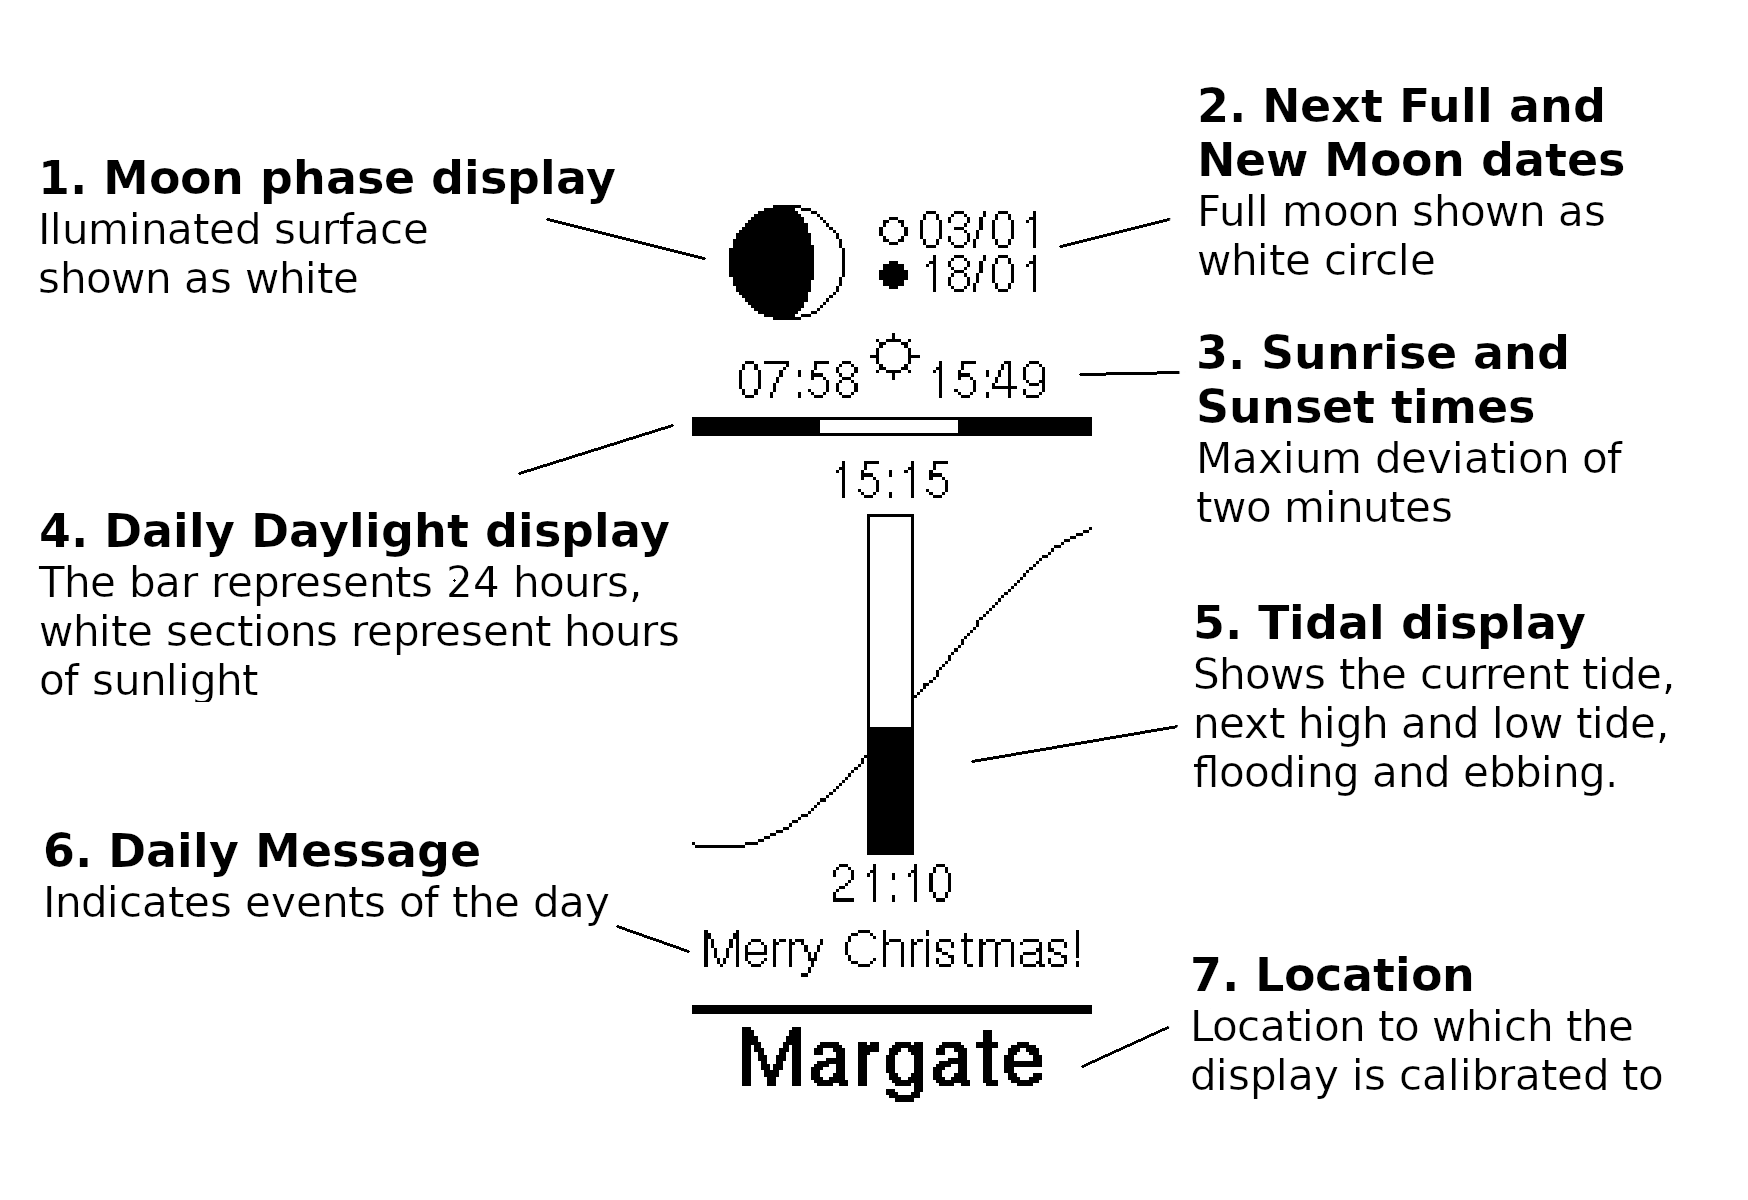
\includegraphics[width=\textwidth,height=0.55\textheight,keepaspectratio]{tidal_screen_anotated.png}

\end{document}
